\documentclass[UTF8,a4paper,11pt,fontset=windows]{ctexart}
\usepackage[margin=22mm,headheight=16pt]{geometry}
\usepackage{amsmath,amssymb,graphicx,array,booktabs,tabularx,longtable}
\usepackage{xcolor,fancyhdr,needspace,float,caption,subcaption}
\usepackage{tikz,enumitem,xurl}
\usetikzlibrary{arrows.meta,positioning,fit,shapes.geometric}
\usepackage[unicode,colorlinks=true,linkcolor=navy,urlcolor=linkblue,citecolor=navy]{hyperref}

\definecolor{navy}{HTML}{173B57}
\definecolor{teal}{HTML}{147D86}
\definecolor{sky}{HTML}{E9F3F7}
\definecolor{mint}{HTML}{E8F5EF}
\definecolor{amber}{HTML}{F4B942}
\definecolor{softamber}{HTML}{FFF5D9}
\definecolor{danger}{HTML}{B84A4A}
\definecolor{linkblue}{HTML}{1769AA}
\definecolor{muted}{HTML}{5E6B73}
\definecolor{linegray}{HTML}{D7DEE3}

\graphicspath{{../../docs/report-assets/progress-20260917/}}
\setlength{\parindent}{0pt}
\setlength{\parskip}{5pt}
\setlength{\emergencystretch}{3em}
\renewcommand{\arraystretch}{1.25}
\raggedbottom
\captionsetup{font=small,labelfont=bf}
\setlist[itemize]{leftmargin=2em,itemsep=2pt,topsep=3pt}
\setlist[enumerate]{leftmargin=2em,itemsep=2pt,topsep=3pt}

\ctexset{
  section={format=\Large\bfseries\color{navy},beforeskip=18pt,afterskip=8pt},
  subsection={format=\large\bfseries\color{teal},beforeskip=12pt,afterskip=5pt}
}

\pagestyle{fancy}
\fancyhf{}
\fancyhead[L]{\small UAV Control Demo}
\fancyhead[R]{\small 铁轨视觉闭环进度报告}
\fancyfoot[L]{\small 2026-09-17}
\fancyfoot[R]{\thepage}
\renewcommand{\headrulewidth}{0.4pt}

\newcommand{\status}[2]{%
  \colorbox{#1}{\parbox[c][1.8em][c]{0.96\linewidth}{\centering\bfseries #2}}}
\newcommand{\githublink}[2]{%
  \par\smallskip
  \noindent\colorbox{sky}{%
    \parbox{\dimexpr\linewidth-2\fboxsep}{%
      \small\textbf{GitHub 链接：}\href{#1}{\textcolor{linkblue}{#2}}}}
  \par\smallskip}
\newcommand{\metric}[2]{%
  \begin{minipage}[t]{0.23\linewidth}
  \centering\colorbox{mint}{\parbox[c][3.6em][c]{0.92\linewidth}{%
  \centering\Large\bfseries\color{navy}#1\\[-1pt]\small\normalfont\color{black}#2}}
  \end{minipage}}
\newcommand{\code}[1]{\texttt{#1}}

\tikzset{
  flow/.style={draw=navy,rounded corners=3pt,fill=sky,minimum height=10mm,
               text width=26mm,align=center,font=\small},
  control/.style={draw=teal,rounded corners=3pt,fill=mint,minimum height=10mm,
                  text width=28mm,align=center,font=\small},
  safety/.style={draw=danger,rounded corners=3pt,fill=red!5,minimum height=9mm,
                 text width=27mm,align=center,font=\small},
  arrow/.style={-{Latex[length=2.4mm]},thick,draw=muted}
}

\begin{document}

\begin{titlepage}
\thispagestyle{empty}
\vspace*{18mm}
{\color{navy}\rule{\linewidth}{1.5pt}}\\[12mm]
{\Huge\bfseries 基于视觉的无人机铁轨循迹\\[4mm]
项目进度报告}\\[8mm]
{\Large YOLO 分割、动态轨面投影与 PX4 闭环验证}\\[12mm]

\begin{center}
\metric{53}{项工程测试}\hfill
\metric{21/21}{闭环识别轮次有效}\hfill
\metric{±0.4 m}{横向边界验证}\hfill
\metric{±10°}{航向边界验证}
\end{center}

\vfill
\begin{minipage}{\linewidth}
\colorbox{softamber}{\parbox{\dimexpr\linewidth-2\fboxsep}{%
\textbf{当前结论。} 直轨 Gazebo/PX4 SITL 中，轨道分割、相机标定、动态单应投影、
米制中心线拟合和有界控制已经形成可重复闭环。正、反两个边界工况均收敛并完成
三次低速前进后确认降落。当前结论不包含真实树莓派、真实相机、人员停车和长距离实飞。}}
\end{minipage}

\vfill
\begin{tabularx}{\linewidth}{@{}lX@{}}
项目仓库 & \href{https://github.com/Yeyu-Tanxue/UAV_control_demo}{%
\textcolor{linkblue}{github.com/Yeyu-Tanxue/UAV\_control\_demo}} \\
报告日期 & 2026-09-17 \\
目标平台 & Raspberry Pi 伴随计算机 + PX4 飞控 \\
当前验证 & Gazebo Harmonic + PX4 SITL + MAVSDK + Spring YOLO 分割 \\
\end{tabularx}
\vspace{8mm}
{\color{navy}\rule{\linewidth}{1.5pt}}
\end{titlepage}

\tableofcontents
\clearpage

\section{项目范围与当前结论}
\githublink{https://github.com/Yeyu-Tanxue/UAV_control_demo/blob/main/README.md}
{仓库主页与当前运行边界}

当前目标被收敛为一个容易验证的最小闭环：
\textbf{悬停 - 本地识别 - 横移/偏航纠正 - 条件满足后低速前进 - 再次悬停}。
道岔识别暂不进入控制主链；人员检测数据准备已存在，但人员停车逻辑尚未并入最新
米制闭环。地面计算机只承担仿真、日志和人工监控，识别和控制决策放在同一伴随
计算进程内。

\begin{figure}[H]
\centering
\begin{tikzpicture}[node distance=8mm and 6mm]
\node[flow] (cam) {相机图像\\640×480};
\node[flow,right=of cam] (yolo) {YOLO 分割\\轨道区域};
\node[control,right=of yolo] (proj) {动态轨面投影\\姿态 + 高度};
\node[control,right=of proj] (fit) {米制中心线\\横偏 + 航向};
\node[flow,below=13mm of fit] (px4) {PX4 / Gazebo\\飞行动力学};
\node[control,left=of px4] (ctrl) {有界速度控制\\前/右/偏航};
\node[safety,left=of ctrl] (gate) {安全门控\\失败即保持/降落};
\draw[arrow] (cam)--(yolo);
\draw[arrow] (yolo)--(proj);
\draw[arrow] (proj)--(fit);
\draw[arrow] (fit)--(ctrl);
\draw[arrow] (ctrl)--(px4);
\draw[arrow] (px4.west) -| (gate.south);
\draw[arrow] (gate.north) |- (cam.south);
\end{tikzpicture}
\caption{当前闭环主链。Gazebo 真值只用于评估，不进入视觉控制。}
\end{figure}

\begin{center}
\begin{tabularx}{0.96\linewidth}{>{\bfseries}p{0.22\linewidth}XX}
\toprule
层级 & 已完成 & 尚未完成 \\
\midrule
算法 & 分割、动态投影、米制轨道几何、速度门控 & 弯道/岔道策略、人员停车融合 \\
仿真 & 双向边界收敛、时间戳真值对齐、安全降落 & 风扰、长距离、多高度动态工况 \\
硬件 & 树莓派入口和 Picamera2 图像源已写入 & 树莓派性能、实体相机标定、Pixhawk 台架 \\
\bottomrule
\end{tabularx}
\end{center}

\section{视觉数据与轨道分割}
\githublink{https://github.com/Yeyu-Tanxue/UAV_control_demo/blob/main/docs/vision/onboard-visual-control.md}
{树莓派本地轨道视觉闭环说明}

数据阶段审计了 RailGoerl24 连续帧，并将 L4R\_NLB 春、秋、冬季标注转换为
YOLO 分割格式。当前仿真采用 Spring 轨道区域分割模型。控制算法不使用 YOLO
外接框的左右坐标，而使用像素级 \code{ego\_track\_area} 掩膜。模型权重和原始
训练集按仓库策略不进入普通 Git 历史。

\begin{figure}[H]
\centering
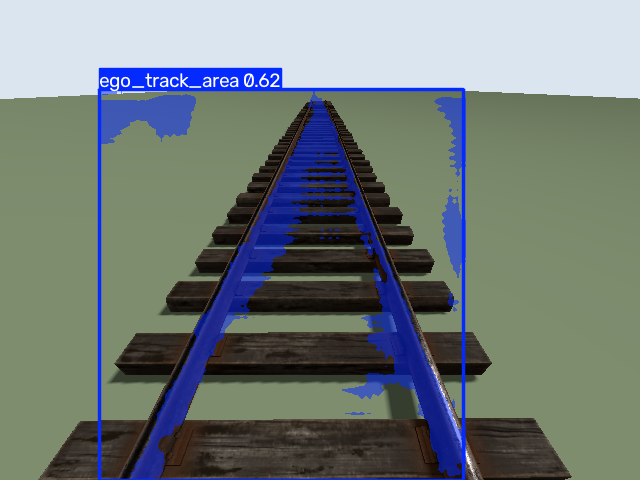
\includegraphics[width=0.82\linewidth]{vision-yolo-segmentation.png}
\caption{Spring YOLO 在直轨 Gazebo 画面上的轨道区域分割。蓝色框只用于显示，
蓝色掩膜才是后续几何计算输入。}
\end{figure}

这一阶段解决了“是否看见当前轨道”的问题，但单靠图像框或掩膜像素中心无法稳定
得到真实米制横偏。为此，后续加入了相机内参、安装位姿、飞行器姿态和距轨面高度，
把分割结果映射到轨面鸟瞰坐标。

\section{直轨 Gazebo 场景与相机模型}
\githublink{https://github.com/Yeyu-Tanxue/UAV_control_demo/blob/main/simulation/gazebo/worlds/rail_demo_realistic.sdf}
{直轨世界、真实轨道模型和 X500 单目相机配置}

当前复现环境由 8 段 4 m 直轨组成。轨道网格实测轨顶高程为
$0.371643$ m，两轨冠中心间距约 $1.592584$ m。相机分辨率为
$640\times480$，水平视场角约 $110^\circ$，固定向前下方 $35^\circ$。
X500 的 \code{base\_link} 高于模型原点 0.24 m，因此相机相对机体位置修正为
FLU 坐标 $(0.12,0,-0.06)$ m。

\begin{figure}[H]
\centering
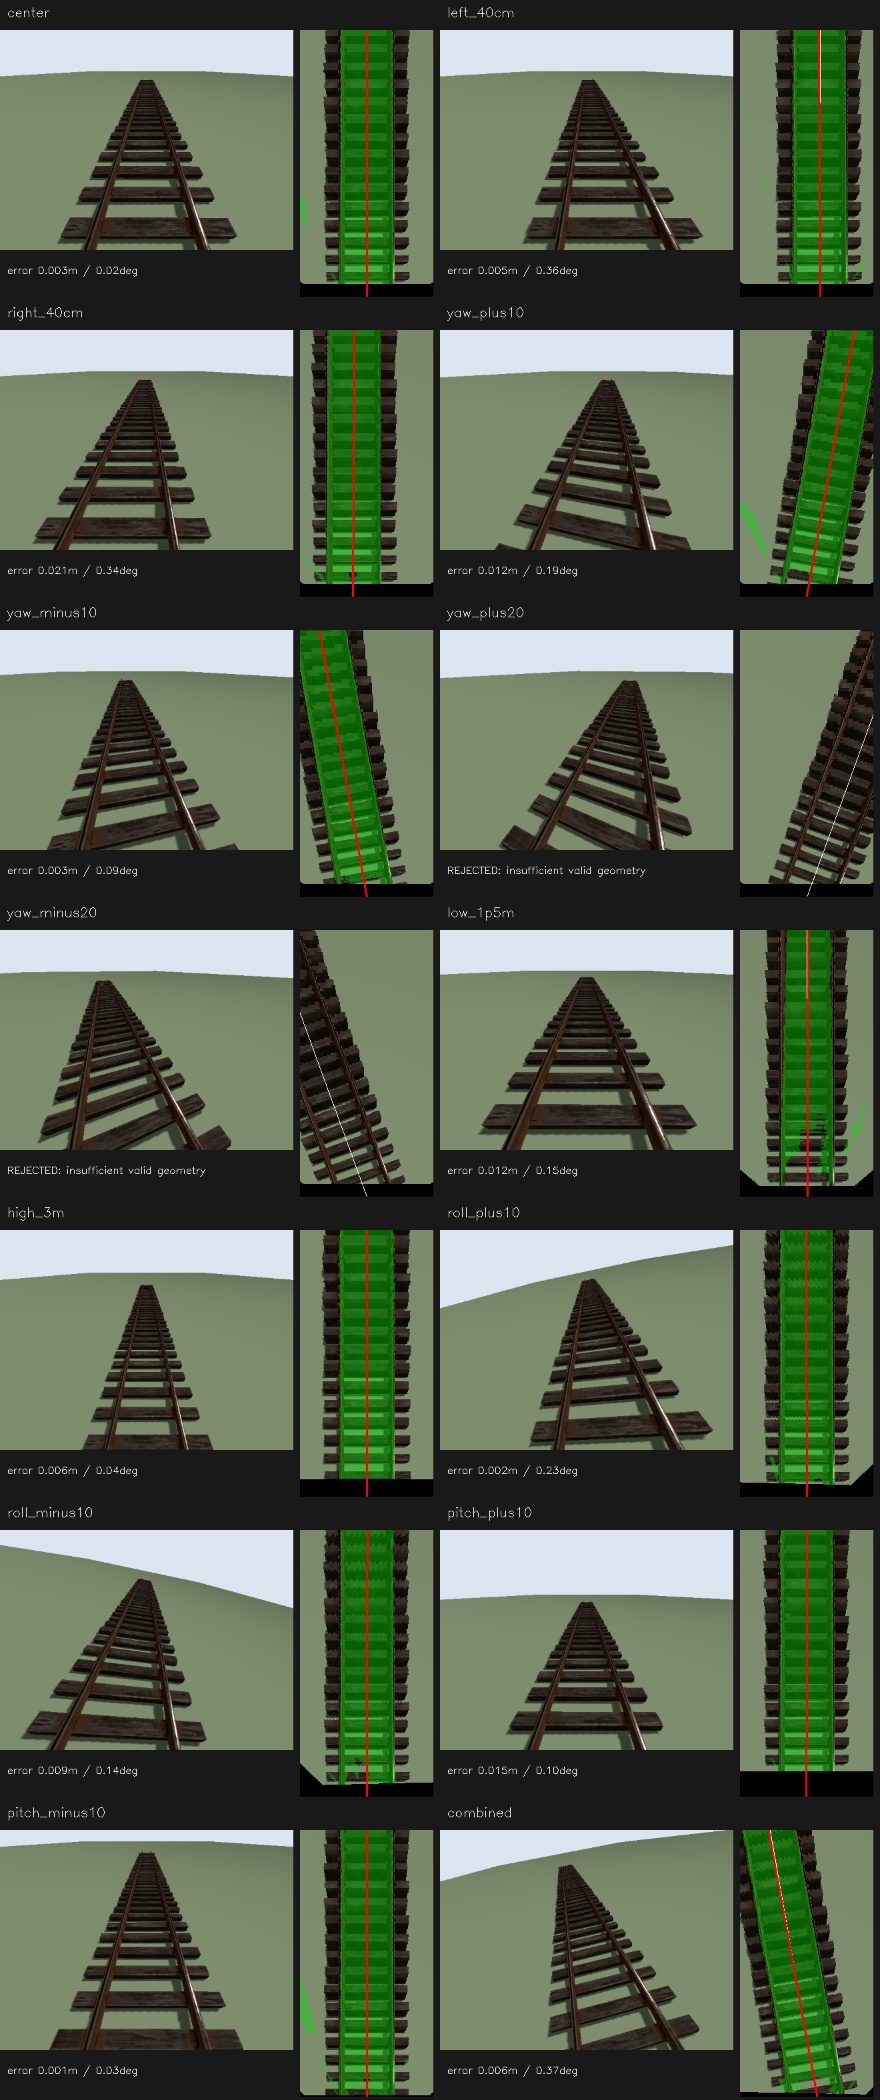
\includegraphics[width=0.93\linewidth,height=0.72\textheight,keepaspectratio]{pose-validation-overview.jpg}
\caption{固定姿态验证总览。图中包含中心、左右偏移、偏航、不同高度、横滚、
俯仰和组合姿态；右侧为轨面鸟瞰与拟合中心线。}
\end{figure}

14 个固定机位中 12 个通过当时设定的 0.10 m / 3° 阈值；有效工况最大横偏误差
约 0.021 m，最大航向误差约 0.37°。旧的 ±2 m 鸟瞰窗口在偏航 ±20° 时拒绝，
后来为边界闭环扩大到左右各 3 m。该拒绝是可观测范围约束，不应解释为模型完全
失效。

\section{相机标定与动态轨面投影}
\githublink{https://github.com/Yeyu-Tanxue/UAV_control_demo/blob/main/src/uav_demo/ground_projection.py}
{动态单应投影实现与像素到鸟瞰米制映射说明}

固定参数包括相机内参 $K$、畸变 $D$ 和相机相对机体的刚性安装变换；
动态参数包括 PX4 的滚转、俯仰以及机体相对轨面的高度。每帧构造轨面到图像的
单应矩阵 $H_g(t)$，再用鸟瞰网格变换 $S$ 得到：
\[
H_{\mathrm{bev}}(t)=S H_g^{-1}(t).
\]
当前鸟瞰范围为前方 0--8 m、左右各 3 m，分辨率 0.02 m/像素。拟合只使用前方
2--6.5 m，并要求轨道宽度、有效行数、前向跨度和残差全部通过检查。

\begin{figure}[H]
\centering
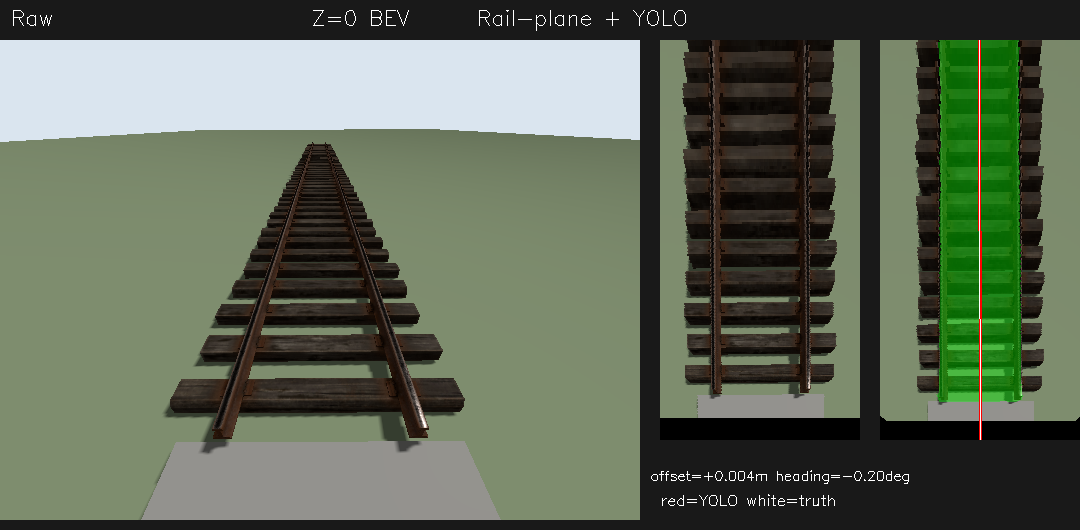
\includegraphics[width=\linewidth]{metric-projection-panel.png}
\caption{左：原始相机图像；中：轨面鸟瞰；右：YOLO 掩膜映射到轨面并拟合
中心线。示例横偏约 $+0.004$ m，航向约 $-0.20^\circ$。}
\end{figure}

Gazebo SITL 现在直接订阅带仿真时间戳的图像消息。评估真值使用同一仿真时间戳
插值；PX4 姿态和高度则按主机接收时钟对图像回调时刻插值。这样避免了早期
“PNG 落盘后再取最新遥测”的主要错位，但实体机仍需硬件时间戳或统一时钟。

\section{米制轨道几何与控制门控}
\githublink{https://github.com/Yeyu-Tanxue/UAV_control_demo/blob/main/src/uav_demo/metric_rail_geometry.py}
{米制轨道拟合、控制映射和安全阈值}

轨道掩膜首先保留最大连通区域，避免离散背景误分割撑宽左右边界。鸟瞰图按行取得
左右边界，中点拟合为
\[
Y(X)=aX+b,\qquad e_y=b,\qquad e_\psi=\arctan(a).
\]
这里 $X$ 是机头水平向前距离，$Y$ 向右为正。控制器采用低增益和明确限幅：

\begin{center}
\begin{tabular}{@{}lll@{}}
\toprule
控制量 & 规则 & 限幅/门槛 \\
\midrule
向右速度 & $v_r=0.55e_y$ & $|v_r|\le0.12$ m/s \\
偏航速度 & $\dot\psi=0.65e_\psi$ & $|\dot\psi|\le6^\circ$/s \\
前进速度 & 连续 3 轮对准后开启 & 0.10 m/s \\
对准条件 & $|e_y|<0.07$ m 且 $|e_\psi|<2^\circ$ & 每轮重新检查 \\
控制包线 & $|e_y|\le0.7$ m 且 $|e_\psi|\le15^\circ$ & 超出即拒绝动作 \\
\bottomrule
\end{tabular}
\end{center}

\begin{figure}[H]
\centering
\begin{tikzpicture}[node distance=6mm]
\node[flow] (mask) {YOLO 掩膜};
\node[flow,right=of mask] (clean) {最大连通区域\\+ 可见范围};
\node[control,right=of clean] (rows) {逐行左右边界\\轨宽筛选};
\node[control,below=of rows] (fit) {鲁棒直线拟合\\残差筛选};
\node[flow,left=of fit] (estimate) {横偏 $e_y$\\航向 $e_\psi$};
\node[safety,left=of estimate] (safe) {门控与限幅\\前进许可};
\draw[arrow] (mask)--(clean);
\draw[arrow] (clean)--(rows);
\draw[arrow] (rows)--(fit);
\draw[arrow] (fit)--(estimate);
\draw[arrow] (estimate)--(safe);
\end{tikzpicture}
\caption{分割掩膜到机体系速度命令的计算顺序。}
\end{figure}

\section{动态闭环验证结果}
\githublink{https://github.com/Yeyu-Tanxue/UAV_control_demo/blob/main/docs/validation/metric-closed-loop-boundary-20260916.md}
{±0.4 m / ±10° 正反边界验证记录与复现入口}

最终验证使用 \code{scripts/run\_metric\_closed\_loop.py}，每轮悬停后获取 3 帧，
至少 2 帧有效才接受，并取横偏和航向的中位数。图像与评估真值按同一 Gazebo
仿真时间戳对齐，真值不输入控制器。

\begin{center}
\begin{tabularx}{0.96\linewidth}{@{}lcc@{}}
\toprule
指标 & 正向工况 & 反向工况 \\
\midrule
实际横偏 & $+0.384\rightarrow+0.031$ m & $-0.358\rightarrow-0.008$ m \\
实际航向 & $+10.51\rightarrow+0.16^\circ$ & $-10.06\rightarrow-0.22^\circ$ \\
有效识别轮次 & 10/10 & 11/11 \\
横偏估计 MAE & 0.012 m & 0.014 m \\
航向估计 MAE & 0.07° & 0.26° \\
高度误差平均/最大 & 0.010/0.030 m & 0.030/0.050 m \\
前进脉冲、降落 & 3 次、确认 & 3 次、确认 \\
异常记录 & 无 & 无 \\
\bottomrule
\end{tabularx}
\end{center}

\begin{figure}[H]
\centering
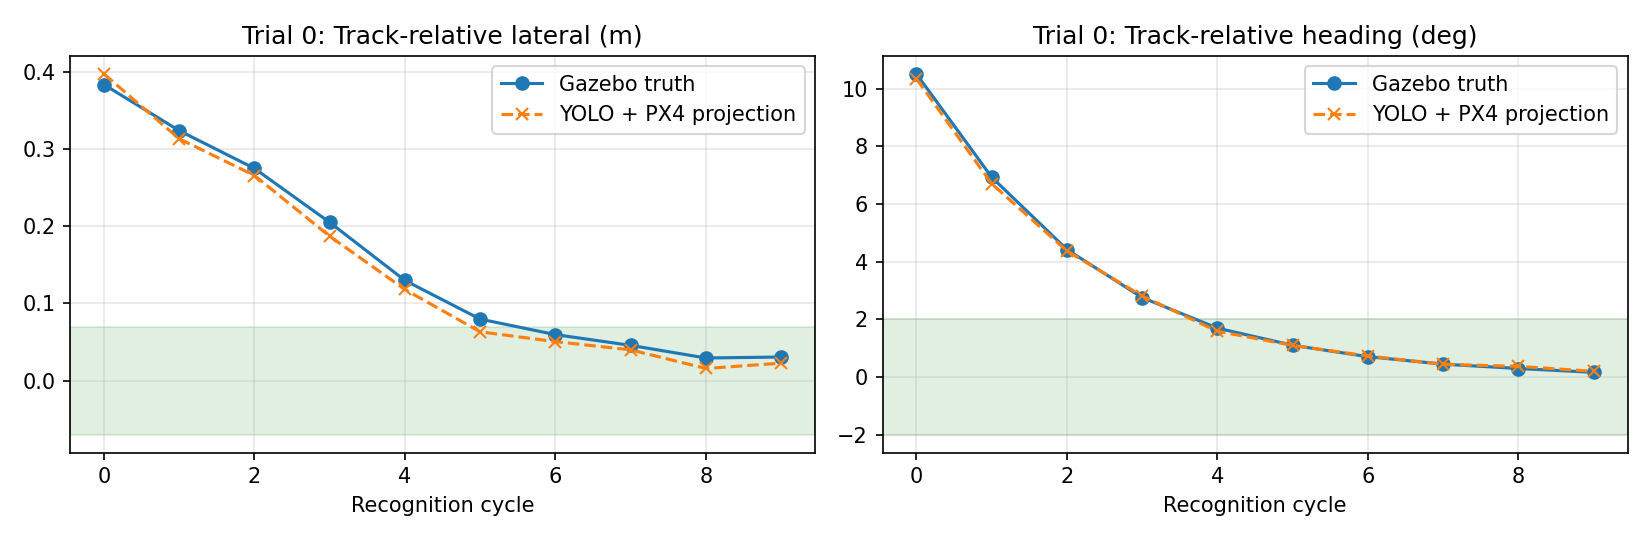
\includegraphics[width=\linewidth]{closed-loop-positive.png}
\caption{正向边界工况。蓝色为 Gazebo 真值，橙色为 YOLO + PX4 动态投影估计；
绿色区域是前进许可阈值。}
\end{figure}

\begin{figure}[H]
\centering
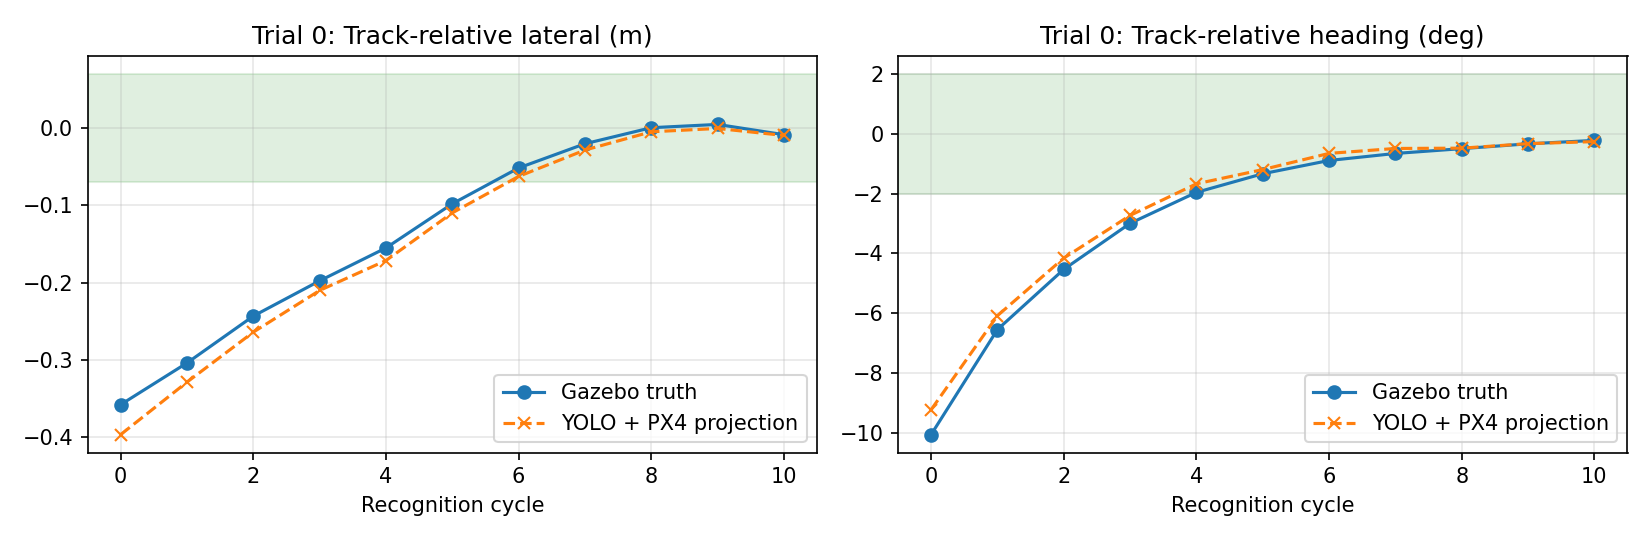
\includegraphics[width=\linewidth]{closed-loop-negative.png}
\caption{反向边界工况。横偏与航向符号均反转，控制器仍稳定收敛。}
\end{figure}

两组结果证明了当前直轨、慢速、单场景下的闭环符号与量级正确；并不能外推到
弯道、强风、快速姿态变化或真实铁路环境。

\section{安全机制与伴随计算机部署}
\githublink{https://github.com/Yeyu-Tanxue/UAV_control_demo/blob/main/src/uav_demo/backends/mavsdk_px4.py}
{MAVSDK/PX4 后端、树莓派图像源和安全降落逻辑}

控制命令为 FRD 机体系速度：前、右、下以及顺时针偏航率。每个 1 s 控制脉冲后
立即发送零速度并重新悬停。连续 3 轮视觉失败、遥测过期、相机帧过期或几何超出
包线都会停止沿用旧命令并进入保护降落。降落超时不会强制解除武装。

\begin{figure}[H]
\centering
\begin{tikzpicture}[node distance=7mm and 10mm]
\node[flow] (hover) {悬停稳定};
\node[flow,right=of hover] (recognize) {本地三帧识别};
\node[control,right=of recognize] (valid) {几何有效?};
\node[control,below=of valid] (pulse) {1 s 有界控制脉冲};
\node[flow,left=of pulse] (zero) {零速度\\重新悬停};
\node[safety,right=of pulse] (land) {连续失败/异常\\安全降落};
\draw[arrow] (hover)--(recognize);
\draw[arrow] (recognize)--(valid);
\draw[arrow] (valid)--node[right,font=\scriptsize]{是}(pulse);
\draw[arrow] (pulse)--(zero);
\draw[arrow] (zero)--(hover);
\draw[arrow] (valid)--node[above,font=\scriptsize]{否}(land);
\end{tikzpicture}
\caption{悬停 - 识别 - 脉冲控制状态机与失败路径。}
\end{figure}

树莓派端已提供 \code{Picamera2FrameSource}、本地 YOLO 入口和串口 MAVSDK 配置。
但目前“树莓派可运行”只停留在软件接口层，尚未完成实体 Pi 5 的帧率、温度、
供电和端到端时延测试。

\section{完成度、限制与下一步}
\githublink{https://github.com/Yeyu-Tanxue/UAV_control_demo/blob/main/docs/simulation/metric-closed-loop.md}
{米制闭环详细说明、已知限制和实体迁移边界}

\begin{figure}[H]
\centering
\begin{tikzpicture}[node distance=5mm]
\node[control] (a) {已完成\\直轨视觉闭环};
\node[control,right=of a] (b) {下一步\\Pi 5 离线推理};
\node[flow,right=of b] (c) {实体相机\\内参/畸变/俯角};
\node[flow,below=of c] (d) {Pi + Pixhawk\\拆桨台架};
\node[safety,left=of d] (e) {人员停车\\失联与接管};
\node[safety,left=of e] (f) {封闭场地\\低高度实飞};
\draw[arrow] (a)--(b);
\draw[arrow] (b)--(c);
\draw[arrow] (c)--(d);
\draw[arrow] (d)--(e);
\draw[arrow] (e)--(f);
\end{tikzpicture}
\caption{从当前 SITL 成果迁移到实体演示的建议顺序。}
\end{figure}

\begin{longtable}{@{}p{0.22\linewidth}p{0.34\linewidth}p{0.34\linewidth}@{}}
\toprule
工作项 & 当前状态 & 验收目标 \\
\midrule
树莓派计算 & 未实测 & 640×480 本地推理至少 2 FPS，持续 30 min 不降频 \\
实体相机 & 未标定 & 获取 $K,D$、安装外参和硬件时间戳 \\
高度来源 & 仿真使用 NED + 初始高程 & 接入下视测距，验证轨面高度误差 \\
Pixhawk 通信 & SITL MAVSDK 已完成 & USB 后转 TELEM2，拆桨验证方向和失联保护 \\
人员检测 & 未并入米制闭环 & 人员出现时停止，连续确认后恢复或降落 \\
连续循迹 & 仅 3 次 0.10 m/s 脉冲 & 长距离、不同高度、风扰和真实纹理 \\
\bottomrule
\end{longtable}

工程测试共 53 项并全部通过。仓库不上传模型权重、原始训练集、完整捕获序列和
PX4 日志；GitHub 中保留可复现代码、场景、精选证据图、验证结论和本报告。

\clearpage
\section*{关键 GitHub 索引}
\addcontentsline{toc}{section}{关键 GitHub 索引}
\begin{itemize}
\item \href{https://github.com/Yeyu-Tanxue/UAV_control_demo/blob/main/scripts/run_metric_closed_loop.py}
{米制闭环试飞入口}
\item \href{https://github.com/Yeyu-Tanxue/UAV_control_demo/blob/main/src/uav_demo/camera_geometry.py}
{相机内参与安装几何}
\item \href{https://github.com/Yeyu-Tanxue/UAV_control_demo/blob/main/src/uav_demo/ground_projection.py}
{动态轨面投影}
\item \href{https://github.com/Yeyu-Tanxue/UAV_control_demo/blob/main/src/uav_demo/metric_rail_geometry.py}
{米制轨道几何}
\item \href{https://github.com/Yeyu-Tanxue/UAV_control_demo/blob/main/src/uav_demo/metric_control.py}
{米制控制映射}
\item \href{https://github.com/Yeyu-Tanxue/UAV_control_demo/blob/main/src/uav_demo/gazebo_transport.py}
{Gazebo 时间戳图像与真值缓冲}
\item \href{https://github.com/Yeyu-Tanxue/UAV_control_demo/blob/main/scripts/run_rpi_vision_demo.sh}
{树莓派运行入口}
\item \href{https://github.com/Yeyu-Tanxue/UAV_control_demo/tree/main/tests}
{测试集}
\end{itemize}

\vfill
\begin{center}
\small\color{muted}
本报告由仓库内 LaTeX 源码生成。数值来自 2026-09-16 保存的两组边界闭环记录。
\end{center}

\end{document}
